\clearpage\secrel{AlgoGraphs:\\Metamodeling in terms of Objects}\secdown

\noindent \term{AlgoGraph} (AG) is a main actor in our system. AG is a
\term{hypergraph} of \emph{interacting} objects (actors). Objects have
\emph{active nature}, so they can \emph{modify} AG itself.

\medskip\noindent
An interaction between objects does via \term{message passing}, which is
\emph{native to distributed systems} and have very good \term{scalability}.

\medskip\noindent
Elements of AG describes widely used elements of software systems, so our model
is mix of \href{http://en.wikipedia.org/wiki/Actor_model}{Actor Model},
\href{http://en.wikipedia.org/wiki/Generic_programming}{Generic Programming}
and \href{http://en.wikipedia.org/wiki/Model-driven_engineering}{Model-driven
engineering} with adaptation for
\href{http://en.wikipedia.org/wiki/Metaprogramming}{Metaprogramming}.

\clearpage\noindent
Ideal structure of final o\F\ system will be:\\
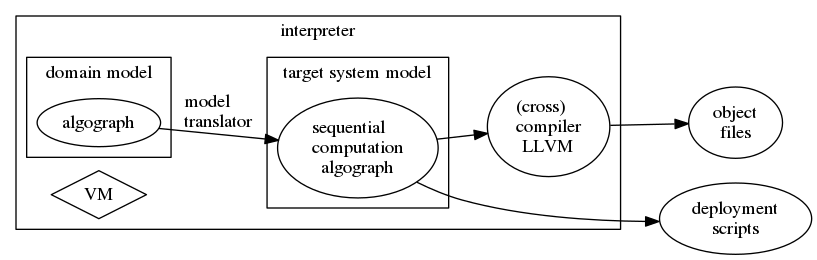
\includegraphics[width=\textwidth]{img/dynamodel.png}\\
\term{Metaprogram} controls build of \term{algograph}, which \emph{describes
required abstract computing system in terms of generic elements}: data
containers, data flows, actors and messages, algorithms, finite automata,
storages, caches,\ldots

\term{Target model} describes required hardware and deployment: platform,
underlying OS, servers interconnection, databases,\ldots

\term{Model translator} transforms maps computational model into sequential form
able to run\note{in multitasking} on required target system.

Resulting sequential model can be transformed into executable code via
\term{dynamic compilaton} \ref{dynacomp}, using LLVM cross-compiler for
required target system, or some mainstream language generators. Also, the
accompanying deployment scripts, packages/installers and other precompiled data
are generated.

% \clearpage
\secrel{Algorithms vs AlgoGraphs}

\noindent
\href{http://en.wikipedia.org/wiki/Algorithm}{Algorithm} is a description of a
\emph{principally sequential process} of doing computations, control, or any
process in general.

\medskip\noindent
\term{AlgoGraph} are is \emph{in principle non-sequential}\note{if you do not
do a special effort on \term{synchronization}}, so it is a second feature to be
good for parallel software systems description and design.

\medskip\noindent
The most buzzword methodologies can be natively described in algographs and AG
itself has the ability to transform models, and especially useful to generate
program code to make designed models be directly used for computations and
production systems design.


\secrel{Actor model vs OOP}

\term{Actor model} is an extrapolation of object oriented programming. In
traditional OOP implementations all messages pass via \emph{synchronous} calls:
do message \verb|object.call(parameters)| and object returns result and
execution \emph{back to call point}. Even in most objected SmallTalk
language messages are sent synchronously.

Contrary to this, actors works asynchronously in principle. Every actor has a
\term{mailbox} (message dispatch entry) and process every message received one
by one. If an actor needs to interact with other it sends the message
asynchronously and continues its job\note{or wait for answer if you need to
mimic classical synchronous processing}.

\clearpage\noindent
Actor can:
\begin{itemize}[nosep]
  \item process incoming messages \emph{sequentially} one by one
  \item send \emph{async} messages to other actors
  \item \emph{create new} actors
  \item \emph{maintain private state} impacts on next messages processing
  \item \emph{mutate its state} as result of procesing message
\end{itemize}

\bigskip\noindent
As you can view \href{https://www.youtube.com/watch?v=7erJ1DV_Tlo}{in this
video}, the actor is primitive computing unit requires these essential 
elements:
\begin{enumerate}[nosep]
  \item processing
  \item storage
  \item communication
\end{enumerate} 
\clearpage\secrel{Advantages of actor model}\secdown

\secrel{Fault tolerance}

\href{http://www.brianstorti.com/the-actor-model/}{Here} you can find a note on
Erlang language as a sample of actor model implementation. Erlang preaches <<let
it crash>> ideology of program development: some actor named \term{process} do
its job without tracking any failure cases can happen when a program executes.
If something goes wrong, the process simply crashes. But this situation will be
caught by another \term{supervisor} actor, which will do crashed process
healing, moving it to some consistent state like just restart the process into
an initial state.
 
\secrel{Scalable computation distribution}

\emph{Message passing is natively scalable} across distributed systems. As all
actors totally \emph{isolated} from each other, there is no matter on what
computing node every actor resides\note{with some overhead of transmitting
messages}. But don't be happy: you still have interprocess data dependency, and
connection link capacity still limits your ability to share your data between
distributed nodes.

\secup
\secup
